\documentclass[tikz,border=5mm]{standalone}
\usetikzlibrary{shapes,calc}

\begin{document}

\newcommand{\ElemLabelL}[4]{
  \begin{minipage}{2.2cm}
   \makebox[\textwidth][lcm]{%
    \textbf{#3}% 元素符号左对齐
    \hfill
   \makebox[0.5cm][r]{%
    \begin{tabular}{@{}r@{}}
      #1 \\ 
      #2    
    \end{tabular}%
  }%
}
    \linebreak\linebreak
    {{#4}}
  \end{minipage}
}

\newcommand{\ElemLabelR}[4]{
  \begin{minipage}{2.2cm}
    \makebox[\textwidth][lcm]{%
      \makebox[0.5cm][l]{%
        \begin{tabular}{@{}l@{}} % 左对齐
          #1 \\ % 第一行显示 #1
          #2    % 第二行显示 #2
        \end{tabular}%
      }%
      \hfill
      \textbf{#3} % 元素符号
    }
    \linebreak \linebreak
    \makebox[\textwidth][r]{{{#4}}} % 元素名称右对齐
  \end{minipage}
}

\newcommand{\Elem}[4]{\ElemLabelL{#1}{#2}{\huge {#3}}{#4}}
\newcommand{\ElemR}[4]{\ElemLabelR{#1}{#2}{\huge {#3}}{#4}}

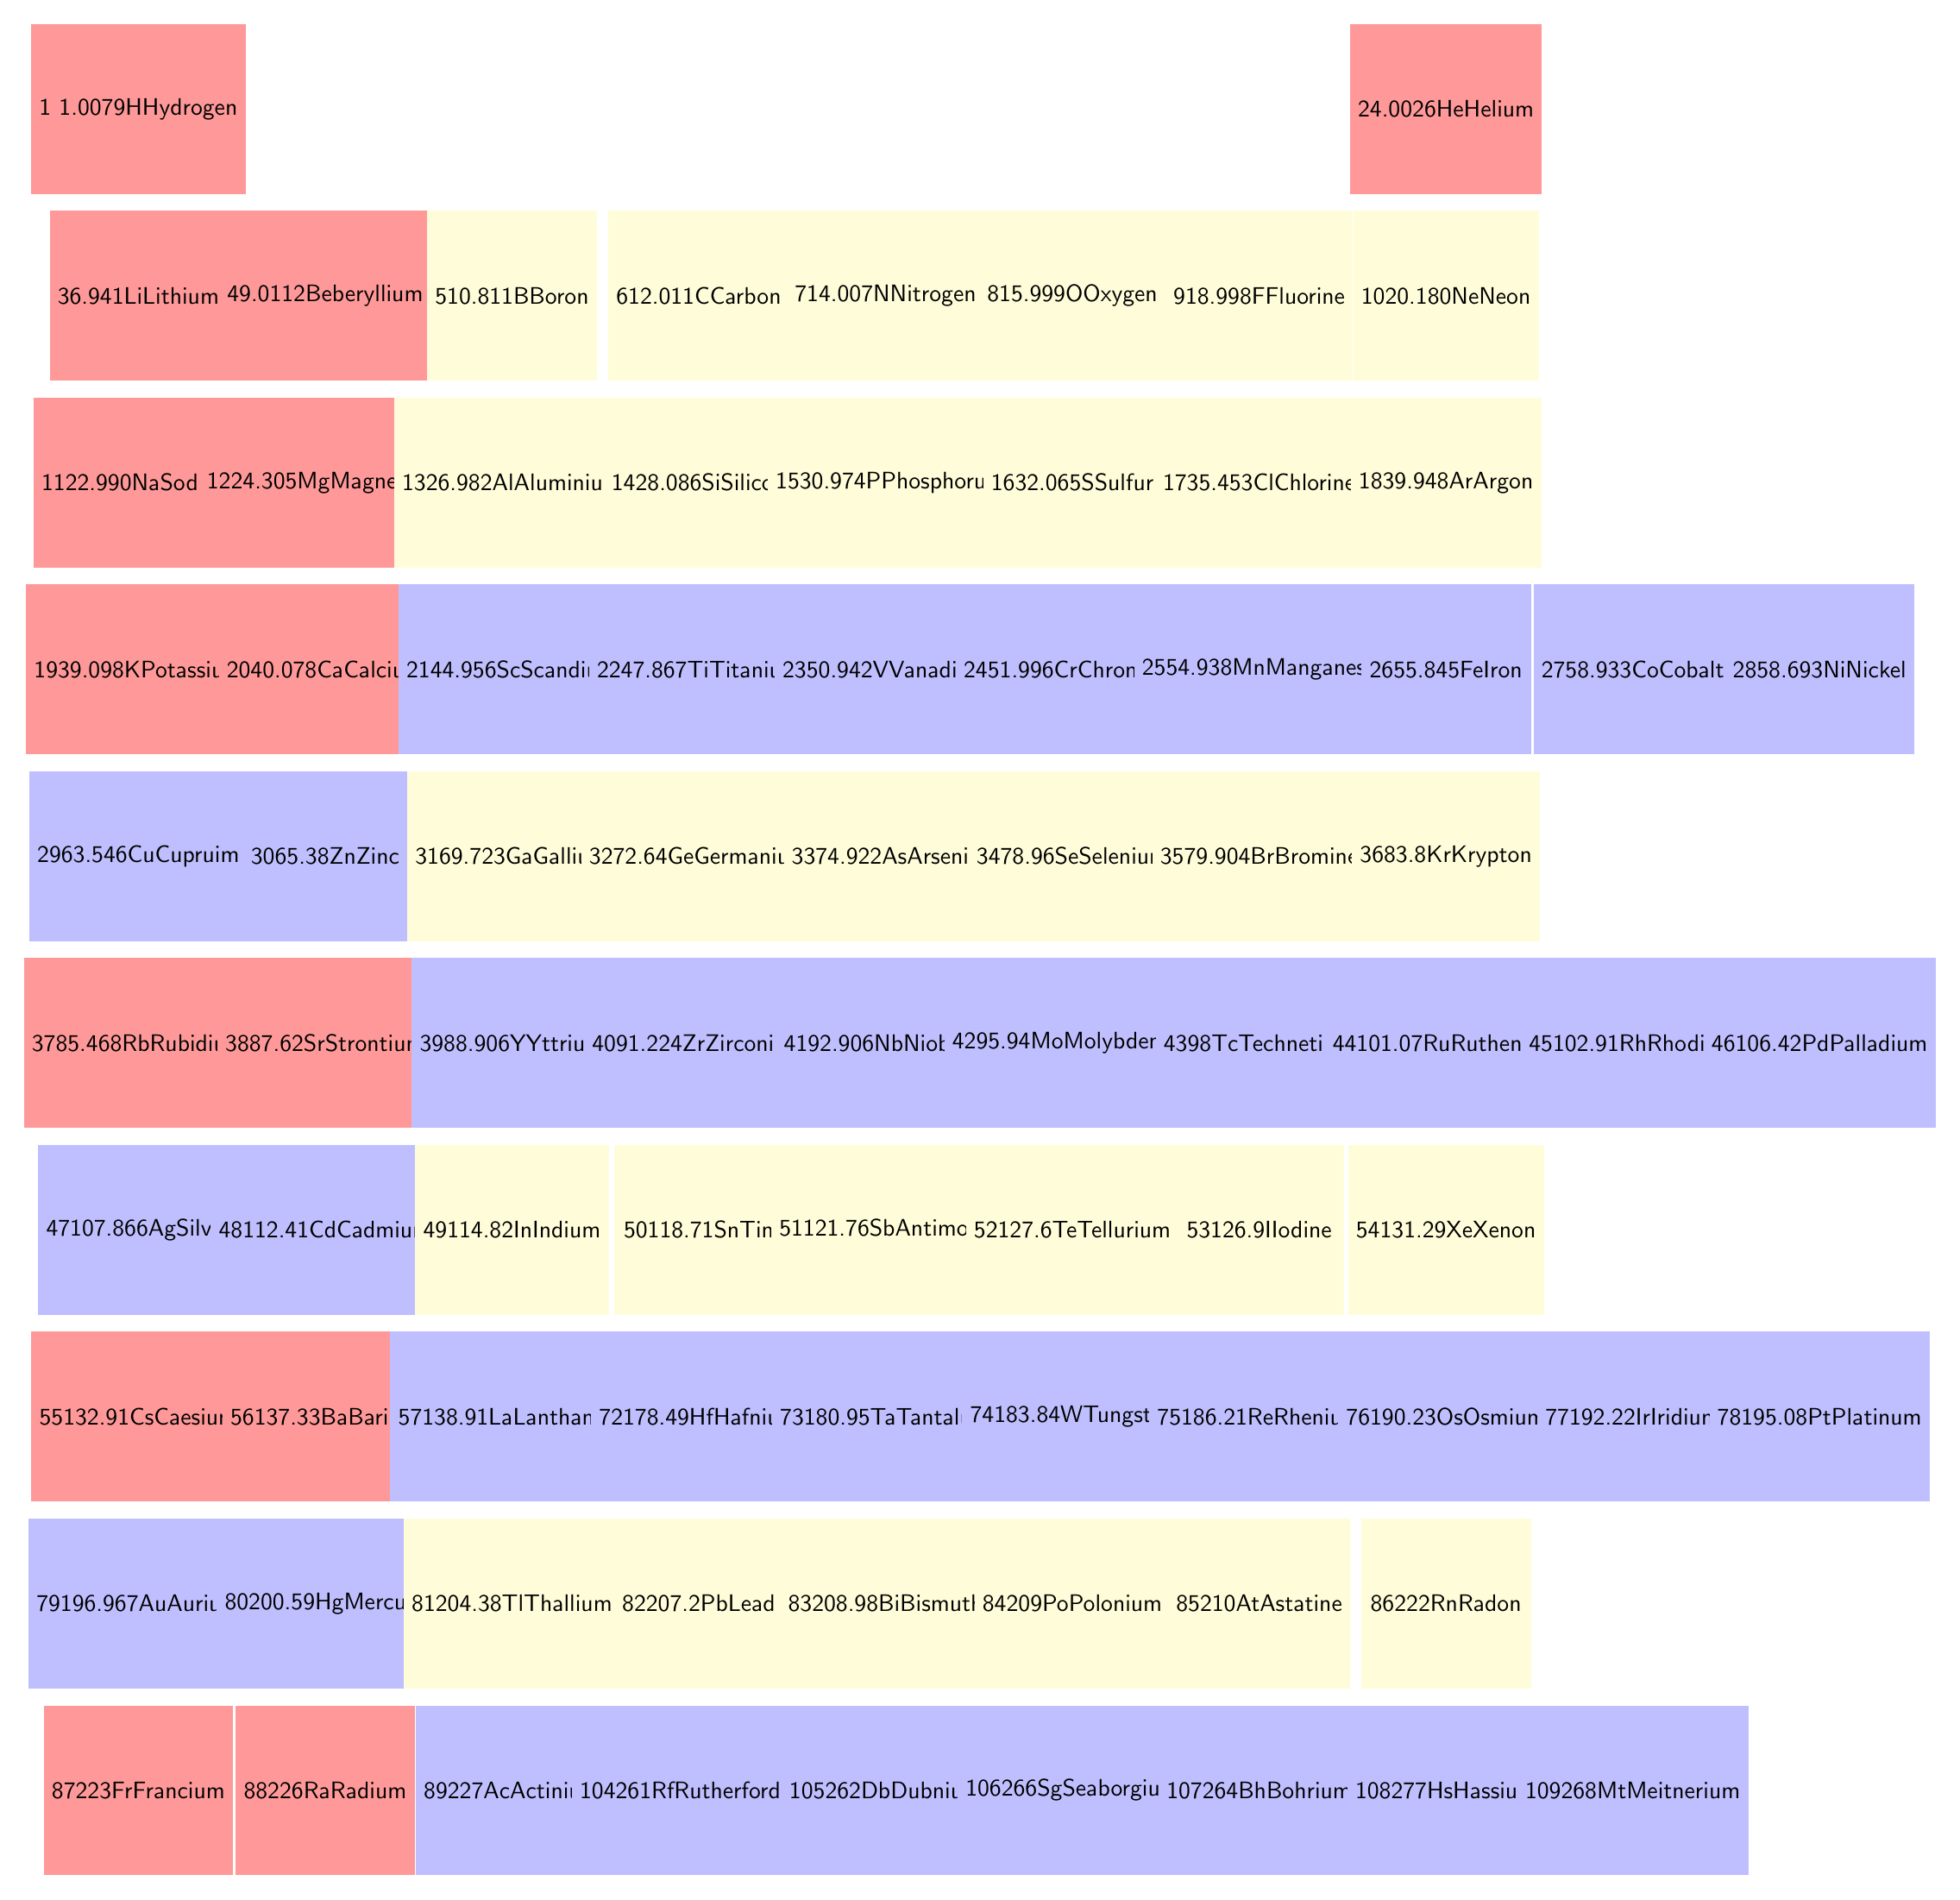
\begin{tikzpicture}[font=\sffamily]
    \tikzstyle{ElementFill_red} = [fill=red!40]
    \tikzstyle{ElementFill_yellow} = [fill=yellow!15]
    \tikzstyle{ElementFill_blue} = [fill=blue!25]

    \tikzstyle{Element_red} = [ElementFill_red,
    minimum width=2.5cm, minimum height=2.5cm, node distance=2.75cm]
    \tikzstyle{Element_yellow} = [ElementFill_yellow,
    minimum width=2.5cm, minimum height=2.5cm, node distance=2.75cm]
    \tikzstyle{Element_blue} = [ElementFill_blue,
    minimum width=2.5cm, minimum height=2.5cm, node distance=2.75cm]

    \node[Element_red] (H) {\Elem{1} {1.0079}{H}{Hydrogen}};
    \node[below of=H, Element_red] (Li) {\Elem{3}{6.941}{Li}{Lithium}};
    \node[below of=Li, Element_red] (Na) {\Elem{11}{22.990}{Na}{Sodium}};
    \node[below of=Na, Element_red] (K) {\Elem{19}{39.098}{K}{Potassium}};
    \node[below of=K, Element_blue] (Cu) {\ElemR{29}{63.546}{Cu}{Cupruim}};
    \node[below of=Cu, Element_red] (Rb) {\Elem{37}{85.468}{Rb}{Rubidium}};
    \node[below of=Rb, Element_blue] (Ag) {\ElemR{47}{107.866}{Ag}{Silver}};
    \node[below of=Ag, Element_red] (Cs) {\Elem{55}{132.91}{Cs}{Caesium}};
    \node[below of=Cs, Element_blue] (Au) {\ElemR{79}{196.967}{Au}{Aurium}};
    \node[below of=Au, Element_red] (Fr) {\Elem{87}{223}{Fr}{Francium}};

    \node[right of=Li, Element_red] (Be) {\Elem{4}{9.0112}{Be}{beryllium}};
    \node[right of=Na, Element_red] (Mg) {\Elem{12}{24.305}{Mg}{Magnesium}};
     \node[right of=K, Element_red] (Ca) {\Elem{20}{40.078}{Ca}{Calcium}};
    \node[right of=Cu, Element_blue] (Zn) {\ElemR{30}{65.38}{Zn}{Zinc}};
    \node[right of=Rb, Element_red] (Sr) {\Elem{38}{87.62}{Sr}{Strontium}};
    \node[right of=Ag, Element_blue] (Cd) {\ElemR{48}{112.41}{Cd}{Cadmium}};
    \node[right of=Cs, Element_red] (Ba) {\Elem{56}{137.33}{Ba}{Barium}};
    \node[right of=Au, Element_blue] (Hg) {\ElemR{80}{200.59}{Hg}{Mercury}};
    \node[right of=Fr, Element_red] (Ra) {\Elem{88}{226}{Ra}{Radium}};

    \node[right of=Be, Element_yellow] (B) {\Elem{5}{10.811}{B}{Boron}};
    \node[right of=Mg, Element_yellow] (Al) {\Elem{13}{26.982}{Al}{Aluminium}};
    \node[right of=Ca, Element_blue] (Sc) {\ElemR{21}{44.956}{Sc}{Scandium}};
    \node[right of=Zn, Element_yellow] (Ga) {\Elem{31}{69.723}{Ga}{Gallium}};
    \node[right of=Sr, Element_blue] (Y) {\ElemR{39}{88.906}{Y}{Yttrium}};
    \node[right of=Cd, Element_yellow] (In) {\Elem{49}{114.82}{In}{Indium}};
    \node[right of=Ba, Element_blue] (La) {\ElemR{57}{138.91}{La}{Lanthanum}};
    \node[right of=Hg, Element_yellow] (Tl) {\Elem{81}{204.38}{Tl}{Thallium}};
    \node[right of=Ra, Element_blue] (Ac) {\ElemR{89}{227}{Ac}{Actinium}};

    \node[right of=B, Element_yellow] (C) {\Elem{6}{12.011}{C}{Carbon}};
    \node[right of=Al, Element_yellow] (Si) {\Elem{14}{28.086}{Si}{Silicon}};
    \node[right of=Sc, Element_blue] (Ti) {\ElemR{22}{47.867}{Ti}{Titanium}};
    \node[right of=Ga, Element_yellow] (Ge) {\Elem{32}{72.64}{Ge}{Germanium}};
    \node[right of=Y, Element_blue] (Zr) {\ElemR{40}{91.224}{Zr}{Zirconium}};
    \node[right of=In, Element_yellow] (Sn) {\Elem{50}{118.71}{Sn}{Tin}};
    \node[right of=La, Element_blue] (Hf) {\ElemR{72}{178.49}{Hf}{Hafnium}};
    \node[right of=Tl, Element_yellow] (Pb) {\Elem{82}{207.2}{Pb}{Lead}};
    \node[right of=Ac, Element_blue] (Rf) {\ElemR{104}{261}{Rf}{Rutherfordium}};

    \node[right of=C, Element_yellow] (N) {\Elem{7}{14.007}{N}{Nitrogen}};
    \node[right of=Si, Element_yellow] (P) {\Elem{15}{30.974}{P}{Phosphorus}};
    \node[right of=Ti, Element_blue] (V) {\ElemR{23}{50.942}{V}{Vanadium}};
    \node[right of=Ge, Element_yellow] (As) {\Elem{33}{74.922}{As}{Arsenic}};
    \node[right of=Zr, Element_blue] (Nb) {\ElemR{41}{92.906}{Nb}{Niobium}};
    \node[right of=Sn, Element_yellow] (Sb) {\Elem{51}{121.76}{Sb}{Antimony}};
    \node[right of=Hf, Element_blue] (Ta) {\ElemR{73}{180.95}{Ta}{Tantalum}};
    \node[right of=Pb, Element_yellow] (Bi) {\Elem{83}{208.98}{Bi}{Bismuth}};
    \node[right of=Rf, Element_blue] (Db) {\ElemR{105}{262}{Db}{Dubnium}};

    \node[right of=N, Element_yellow] (O) {\Elem{8}{15.999}{O}{Oxygen}};
    \node[right of=P, Element_yellow] (S) {\Elem{16}{32.065}{S}{Sulfur}};
    \node[right of=V, Element_blue] (Cr) {\ElemR{24}{51.996}{Cr}{Chromium}};
    \node[right of=As, Element_yellow] (Se) {\Elem{34}{78.96}{Se}{Selenium}};
    \node[right of=Nb, Element_blue] (Mo) {\ElemR{42}{95.94}{Mo}{Molybdenum}};
    \node[right of=Sb, Element_yellow] (Te) {\Elem{52}{127.6}{Te}{Tellurium}};
    \node[right of=Ta, Element_blue] (W) {\ElemR{74}{183.84}{W}{Tungsten}};
    \node[right of=Bi, Element_yellow] (Po) {\Elem{84}{209}{Po}{Polonium}};
    \node[right of=Db, Element_blue] (Sg) {\ElemR{106}{266}{Sg}{Seaborgium}};

    \node[right of=O, Element_yellow] (F) {\Elem{9}{18.998}{F}{Fluorine}};
    \node[right of=S, Element_yellow] (Cl) {\Elem{17}{35.453}{Cl}{Chlorine}};
    \node[right of=Cr, Element_blue] (Mn) {\ElemR{25}{54.938}{Mn}{Manganese}};
    \node[right of=Se, Element_yellow] (Br) {\Elem{35}{79.904}{Br}{Bromine}};
    \node[right of=Mo, Element_blue] (Tc) {\ElemR{43}{98}{Tc}{Technetium}};
    \node[right of=Te, Element_yellow] (I) {\Elem{53}{126.9}{I}{Iodine}};
    \node[right of=W, Element_blue] (Re) {\ElemR{75}{186.21}{Re}{Rhenium}};
    \node[right of=Po, Element_yellow] (At) {\Elem{85}{210}{At}{Astatine}};
    \node[right of=Sg, Element_blue] (Bh) {\ElemR{107}{264}{Bh}{Bohrium}};

    \node[right of=F, Element_yellow] (Ne) {\Elem{10}{20.180}{Ne}{Neon}};
    \node[above of=Ne, Element_red] (He) {\Elem{2}{4.0026}{He}{Helium}};
    \node[right of=Cl, Element_yellow] (Ar) {\Elem{18}{39.948}{Ar}{Argon}};
    \node[right of=Mn, Element_blue] (Fe) {\ElemR{26}{55.845}{Fe}{Iron}};
    \node[right of=Br, Element_yellow] (Kr) {\Elem{36}{83.8}{Kr}{Krypton}};
    \node[right of=Tc, Element_blue] (Ru) {\ElemR{44}{101.07}{Ru}{Ruthenium}};
    \node[right of=I, Element_yellow] (Xe) {\Elem{54}{131.29}{Xe}{Xenon}};
    \node[right of=Re, Element_blue] (Os) {\ElemR{76}{190.23}{Os}{Osmium}};
    \node[right of=At, Element_yellow] (Rn) {\Elem{86}{222}{Rn}{Radon}};
    \node[right of=Bh, Element_blue] (Hs) {\ElemR{108}{277}{Hs}{Hassium}};

    \node[right of=Fe, Element_blue] (Co) {\ElemR{27}{58.933}{Co}{Cobalt}};
    \node[right of=Co, Element_blue] (Ni) {\ElemR{28}{58.693}{Ni}{Nickel}};
    \node[right of=Ru, Element_blue] (Rh) {\ElemR{45}{102.91}{Rh}{Rhodium}};
    \node[right of=Rh, Element_blue] (Pd) {\ElemR{46}{106.42}{Pd}{Palladium}};
    \node[right of=Os, Element_blue] (Ir) {\ElemR{77}{192.22}{Ir}{Iridium}};
    \node[right of=Ir, Element_blue] (Pt) {\ElemR{78}{195.08}{Pt}{Platinum}};
    \node[right of=Hs, Element_blue] (Mt) {\ElemR{109}{268}{Mt}{Meitnerium}};

  
\end{tikzpicture}

\end{document}